\section{Theorie}
\label{sec:Theorie}
Um elektrischen Bauteilen Energie zuzuführen, wird eine Spannungsquelle, beispielsweise ein Dynamo oder ein LC-Generator, benutzt.
In der Theorie wird immer von einer idealen Spannungsquelle ausgegangen, dessen Innenwiderstand über einen zusätzlichen Widerstand $R_i$ realisiert wird.
Um nun in der Praxis Spannungsquellen zu benutzen, müssen die technischen Daten eben dieser bekannt sein.
Es handelt sich um die Leerlaufspannung $U_0$ und den vorhin bereits erwähnten Innenwiderstand $R_i$.\\
Die Leerlaufspannung $U_0$ liegt an einer Spannungsquelle genau dann an, wenn ihr keine Leistung entnommen wird, also bei eingeschalteter Spannungsquelle kein Strom fließt.
Sobald aber ein Strom über einen Lastwiderstand $R_a$ fließt, wie beispielsweise in Abbildung \ref{fig:t1}, wird ein Sinken der Spannung $U_k$ (Klemmspannung) parallel zur Spannungsquelle beobachtet.

\begin{figure}[H]
  \centering
  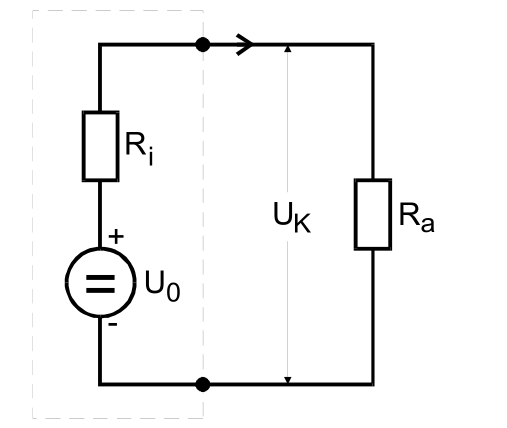
\includegraphics[height=6cm]{innenwiderstand.png}
  \caption{Beispielaufbau \cite{sample}}
  \label{fig:t1}
\end{figure}

Dies folgt aus den Kirchhoffschen Regeln, vorallem aus der Maschenregel (\ref{eqn:maschenregel}).\\
Die Knotenregel folgt direkt aus der Ladungserhaltung und besagt, dass in jedem Knotenpunkt einer Schaltung die Summe aller eingehenden und ausgehenden Ströme verschwinden muss:

\begin{equation}
  \sum_{k=1}^n I_k = 0.
  \label{eqn:knotenregel}
\end{equation}

\begin{figure}[H]
  \centering
  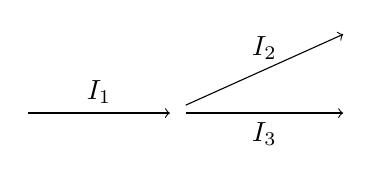
\begin{tikzpicture}
    \draw[->] (0, 0) -- (1.8, 0) node[midway, above] {$I_1$};
    \draw[->] (2, 0.1) -- (4, 1) node[midway, above] {$I_2$};
    \draw[->] (2, 0) -- (4, 0) node[midway, below] {$I_3$};
    %\draw[IPfeil=0em]([yshift=1.0em]0,0) -- node [above]{I$\mathsf{_R}$}([yshift=1.0em]0.5,0);
  \end{tikzpicture}
  \caption{Knotenregel.}
  \label{fig:knotenregel}
\end{figure}

Die zweite und hier tragende Regel ist die Maschenregel.
Sie besagt, dass in jeder geschlossenen Masche der Schaltung die Summe der Spannungen null ergeben muss:
\begin{equation}
  \sum_{i=1}^n U_i = 0.
  \label{eqn:maschenregel}
\end{equation}
Demnach folgt für den Beispielaufbau \ref{fig:t1}, dass die Spannungsquelle einen Innenwiderstand $R_i$ haben muss, der sich in der Formel
\begin{equation}
  U_0 = IR_i + IR_a
\end{equation}
äußert, wobei die oben genannte Klemmenspannung
\begin{equation}
  U_k = IR_a = U_0 - IR_i
  \label{eqn:klemmspannung}
\end{equation}
beträgt.
Dass durch alle Bauteile der selbe Strom fließt, folgt aus der Knotenregel (\ref{eqn:knotenregel}).\\
Würde es den Innenwiderstand nicht geben, folgt aus dem Ohmschen-Gesetz,
\begin{equation}
  U = RI,
\end{equation}
dass mit der Spannungsquelle eine unendlich große Stromstärke $I$ und somit eine beliebig große Leistung $P$ erreicht wird, da für sie
\begin{equation}
  P = I²R_a
  \label{eqn:leistung}
\end{equation}
gilt.
Im realen Fall durchläuft $P(R_a)$ ein Maximum.
Es wird von Leistungsanpassung gesprochen, wenn $R_a$ so gewählt wird, dass die Leistung $P$ der Spannungsquelle maximal wird.
